\documentclass[11pt,a4paper]{article}

\usepackage[margin=2.5cm]{geometry}
\usepackage[T1]{fontenc}
\usepackage{lmodern}
\usepackage{parskip}
\usepackage{enumitem}
\usepackage{graphicx}
\usepackage{subcaption}
\usepackage{booktabs}
\usepackage{tabularx}
\usepackage{xurl}
\usepackage[hidelinks]{hyperref}

\graphicspath{{figures/}}
\newcommand{\videourl}{https://youtu.be/lvxSxMR5IOQ}

\begin{document}

\begin{center}
  {\Large\bfseries BAScii Generative AI -- Final Project Report}\\[0.4em]
  {\large Final Outcome, Demonstration and Reflection}
\end{center}

\vspace{1em}

\begin{tabular}{@{}lp{10.8cm}@{}}
  \textbf{Project Title:}      & Yapperton \\
  \textbf{Group:}              & Aliens \\
  \textbf{Team Members:}       & Wilhelm Axel Durelius (6901009256) \\
                               & Shayan Gardan Gardawan (6901005756) \\
                               & Schahab Bashar-Mal (6901001156) \\
  \textbf{Project Repository:} & \url{https://github.com/schahab04-cpu/chula_class_ollama-codex_local_LLM} \\
  \textbf{Demonstration Video:} & \url{\videourl} \\
\end{tabular}

\vspace{2em}

\section{Project Overview}

Yapperton is an oral study buddy that you can talk with. You upload your course
material, like lecture slides or PDFs, and then you can ask questions about it
and get easy summaries back, either in text or with your voice. Everything runs
locally on the own computer with Ollama, so no documents is sent away to some
company in the cloud. The idea came from that we all three study better when we
explain things out loud to each other, but it is not always that you have a
friend who has time to listen at 11 in the evening the day before the exam.

Our original objectives were: (1) a chat where you ask questions about your own
uploaded documents and get plain-language answers with sources, (2) a
hands-free voice mode with Whisper and Kokoro, (3) everything local with a small
model (qwen3:1.7b) on a normal laptop, and (4) short and easy answers that feel
like a conversation.

\section{Final Outcome and Demonstration}

\subsection*{The completed deliverable}

The final deliverable is a working local web app, Yapperton, that a student
starts on their own laptop with one command (\texttt{python app.py}) and opens
at \texttt{http://127.0.0.1:5050}. The voice screen is the main page: you press
\emph{Start talking} and just talk. A glowing animated ``wisp'' shows what
Yapperton is doing (listening, thinking, speaking, reading a document), and the
latest question and answer are shown as text under it. A text chat and a
document manager are one click away under \emph{Chat \& documents}.

Behind the page is a Flask backend in Python with a retrieval-augmented
generation (RAG) pipeline. Uploaded documents are split into passages, embedded
with \texttt{nomic-embed-text} and stored in a local SQLite index. Questions
are answered by \texttt{qwen3.5:9b} running in Ollama, using the passages that
a hybrid search finds. Voice uses Silero VAD in the browser to hear when you
speak, Whisper (large-v3-turbo) to turn speech into text, and Kokoro to speak
the answer. All four models run on the laptop; nothing needs a cloud account or
a subscription. The project has about 5,800 lines of code and 164 automated
unit tests.

\subsection*{Key features and capabilities}

\begin{itemize}[leftmargin=*]
  \item \textbf{Talk to your slides.} Ask about an uploaded lecture out loud and
        hear the answer. The answer streams sentence by sentence, so the first
        sentence is spoken while the rest is still being written.
  \item \textbf{Answers with sources.} Every answer from a document shows the
        file and page it came from (for example
        ``From GAI\_Literacy\_Lecture\_1.pdf, Page~16''), and in the text chat
        you can open the source passage and the PDF itself.
  \item \textbf{Quizzes on demand.} ``Make a three question quiz about
        predictive and generative AI'' creates multiple-choice questions from
        the documents. Clicking an option shows if it was right, an explanation
        and the source page. Each question is checked by the model a second
        time, and questions with giveaways or ``all of the above'' options are
        removed in code.
  \item \textbf{Attach by voice.} Saying ``I need to attach a document'' opens
        an upload box right on the voice screen. Yapperton then reads the
        document (it pauses while doing so) and is ready for questions.
  \item \textbf{Smart routing.} Course questions are answered from the
        documents, while small talk and general questions get a normal reply.
        Clear cases are decided by rules in code, and unclear ones by asking
        Qwen with a short summary of every uploaded document.
  \item \textbf{Follow-up questions} keep the context of the last answer, and in
        the text chat a doubt like ``is that right?'' starts a fact check on
        Wikipedia with DuckDuckGo as fallback (the only feature that uses the
        internet, and only the question is sent).
  \item \textbf{Formats and safety.} PDF, DOCX, TXT and MD up to 20~MiB;
        duplicate uploads are detected by a SHA-256 fingerprint; uploaded text
        is treated as data, never as instructions; voice audio is never saved.
\end{itemize}

\subsection*{Screenshots and supporting material}

Figure~\ref{fig:screens} shows the app during the recorded demonstration and the
text chat with its document manager. The infographic in
Figure~\ref{fig:infographic} (last page) summarizes the whole application: the
three pipelines, the features, the models and software, the main numbers and
the limits.

\begin{figure}[htbp]
  \centering
  \begin{subfigure}[t]{0.49\textwidth}
    \centering
    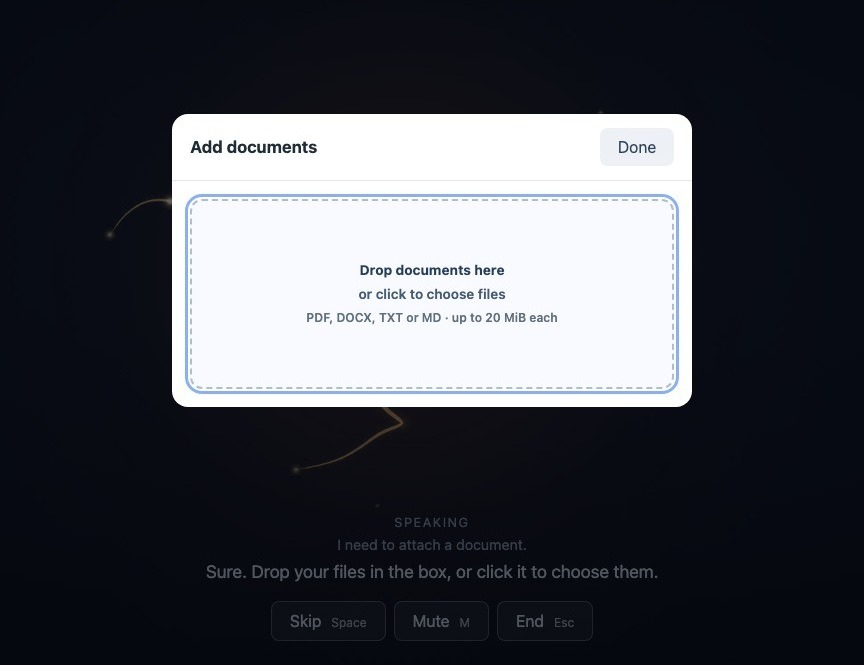
\includegraphics[width=\linewidth]{upload_crop.jpg}
    \caption{``I need to attach a document'' opens the upload box in voice mode.}
  \end{subfigure}\hfill
  \begin{subfigure}[t]{0.49\textwidth}
    \centering
    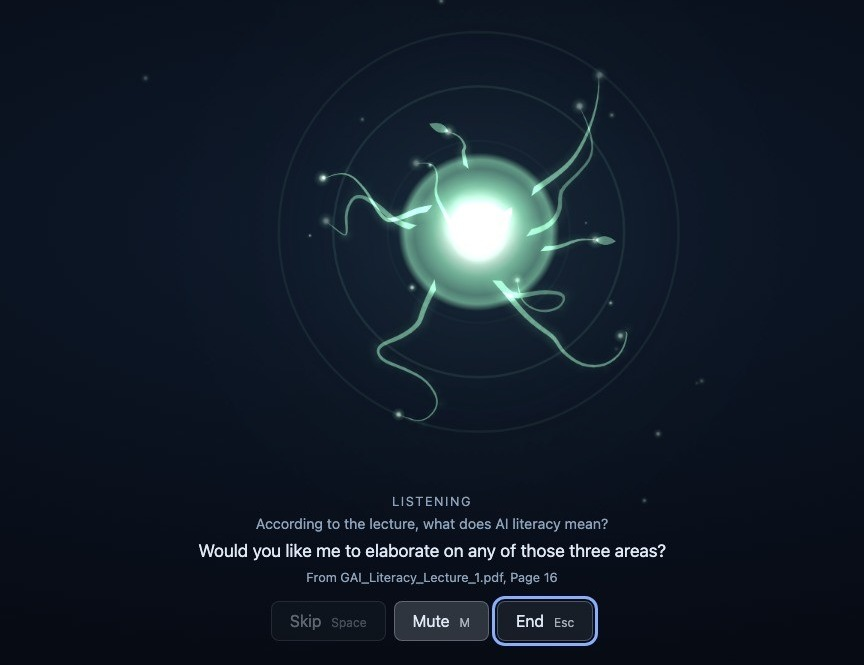
\includegraphics[width=\linewidth]{answer_crop.jpg}
    \caption{A spoken answer about the lecture, with the source page under it.}
  \end{subfigure}

  \vspace{0.8em}
  \begin{subfigure}[t]{0.33\textwidth}
    \centering
    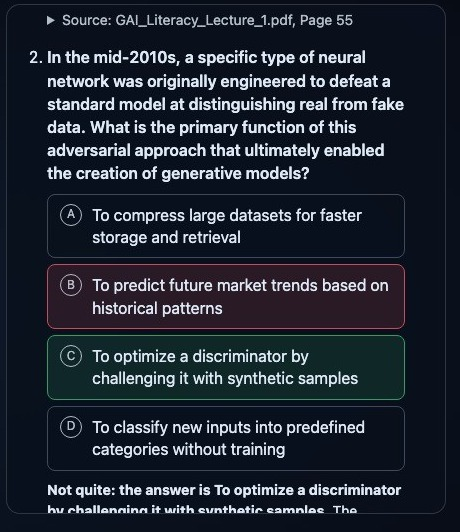
\includegraphics[width=\linewidth]{quiz_panel.jpg}
    \caption{Quiz made by voice: a wrong click (red), the right answer (green), explanation and source.}
  \end{subfigure}\hfill
  \begin{subfigure}[t]{0.63\textwidth}
    \centering
    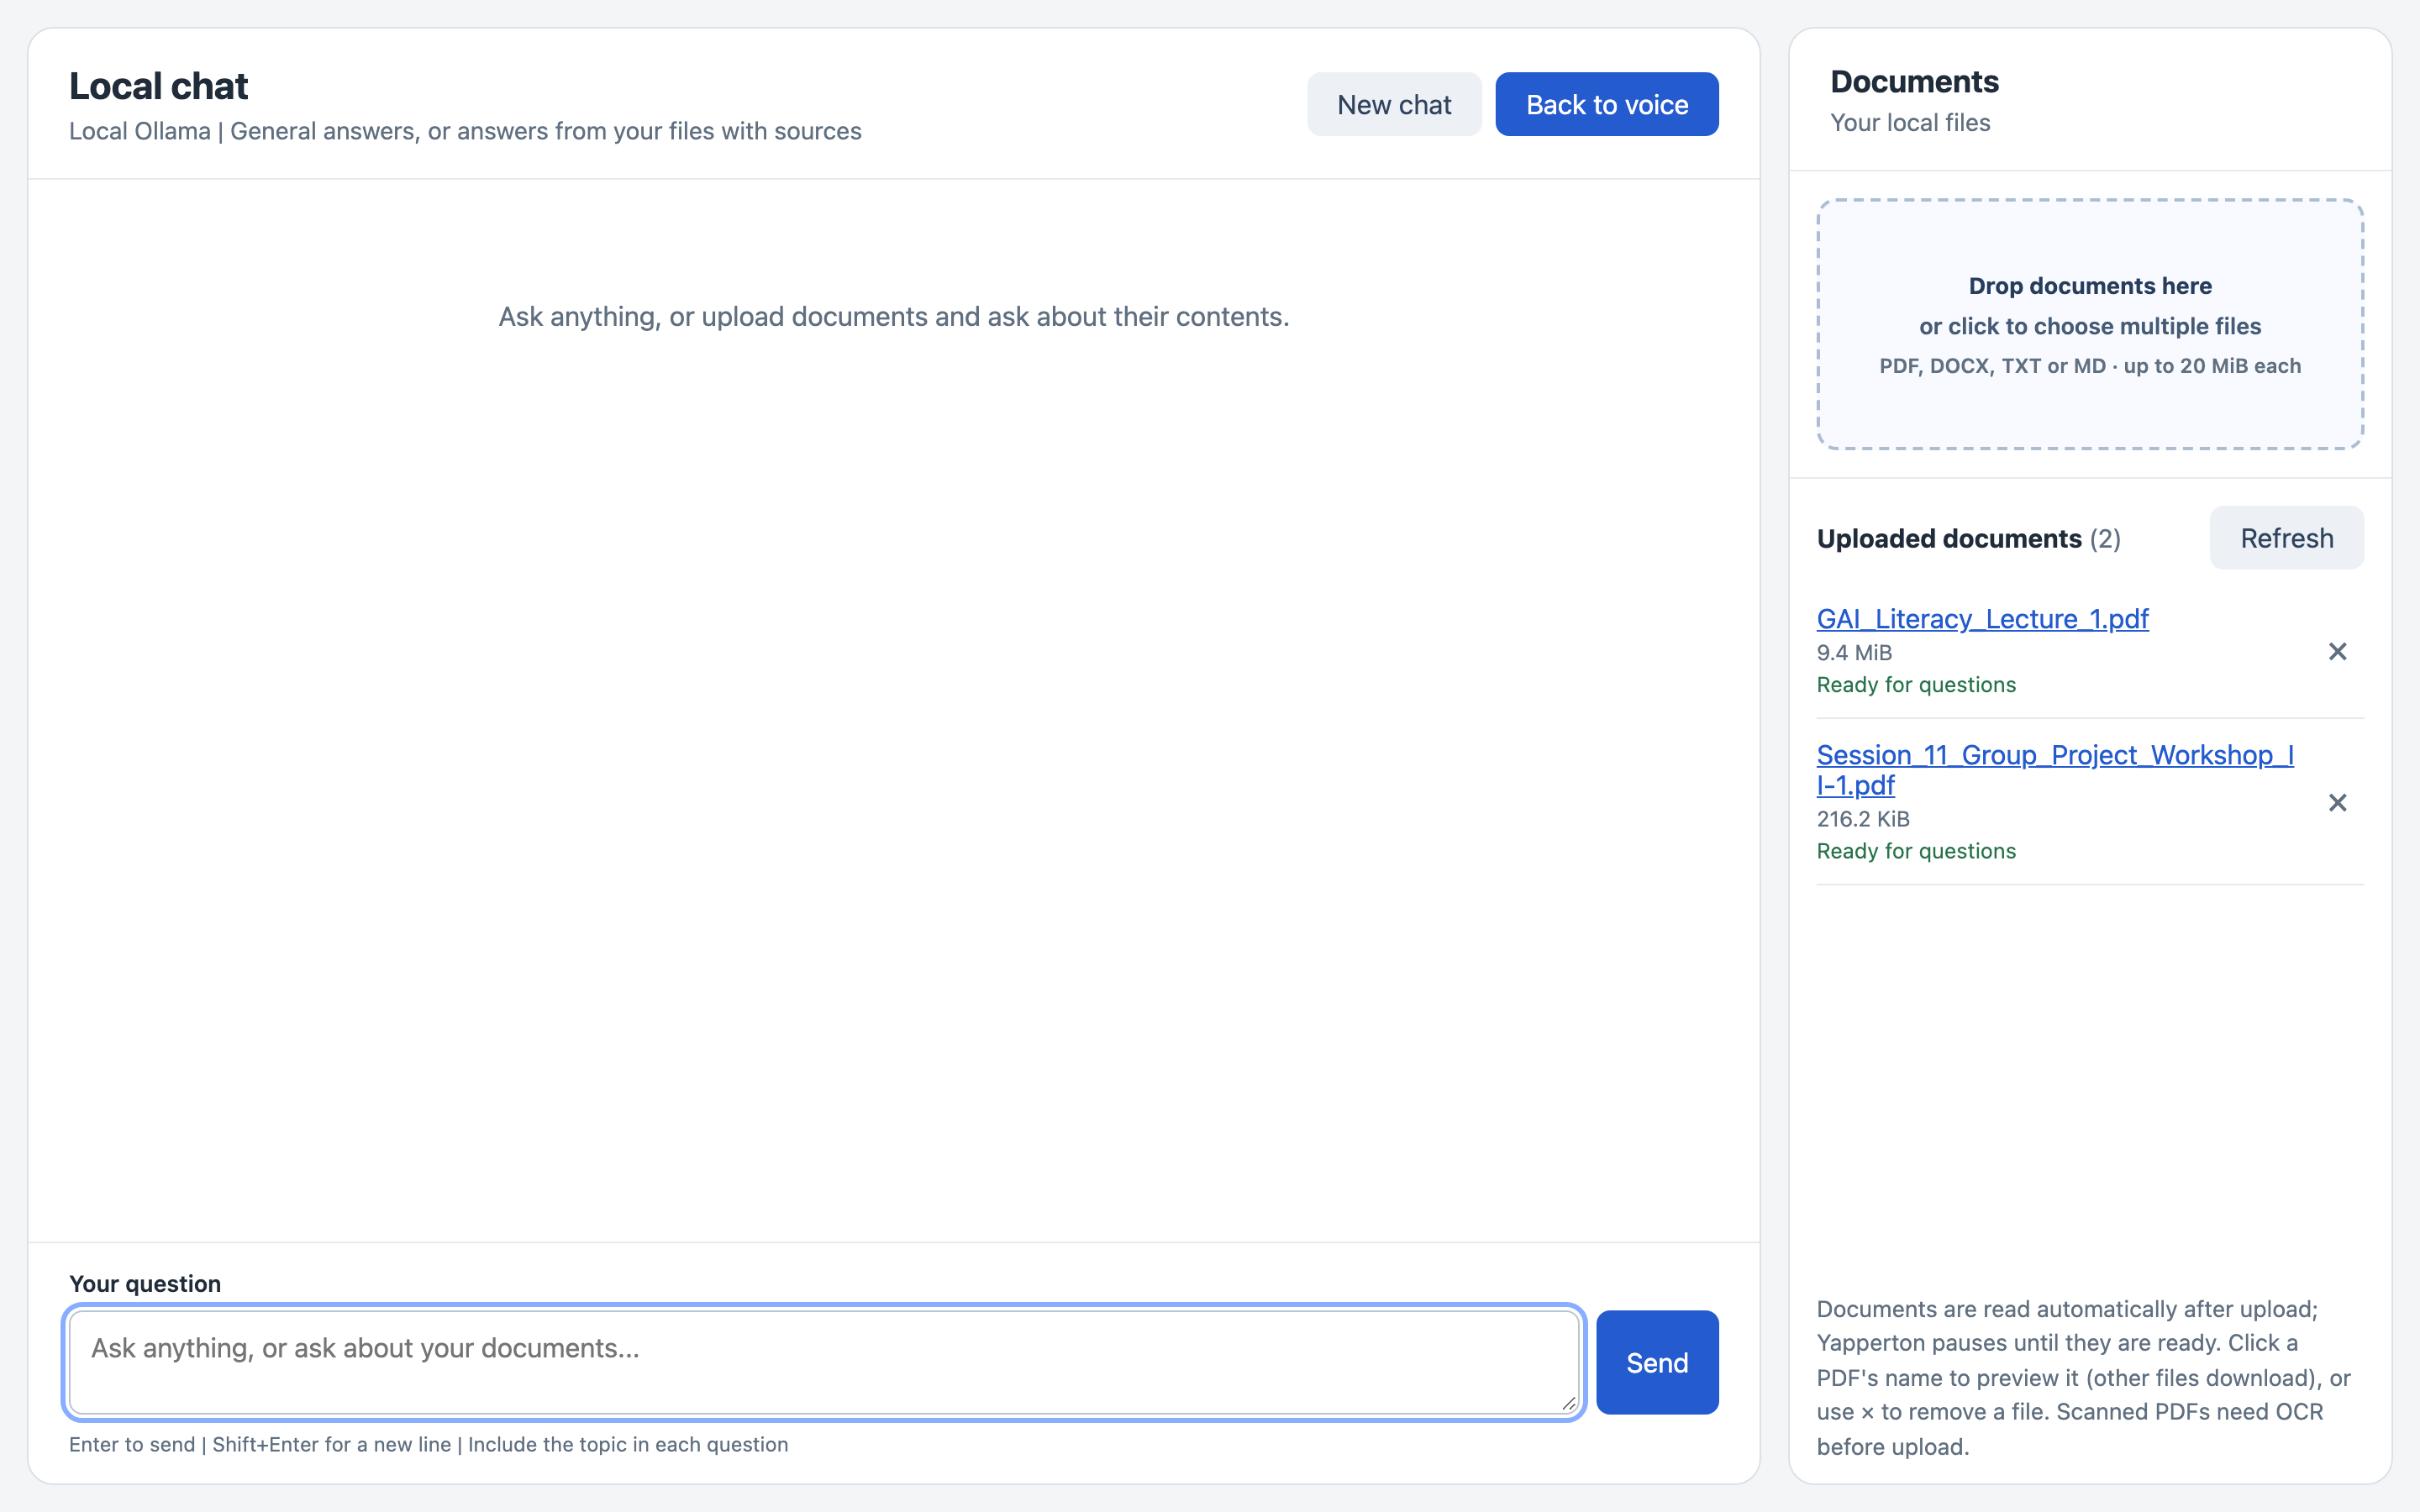
\includegraphics[width=\linewidth]{chat_documents.png}
    \caption{\emph{Chat \& documents}: text chat with sources beside the uploaded documents.}
  \end{subfigure}
  \caption{Yapperton in use. (a)--(c) are frames from the demonstration video;
           the document is the course's GAI Literacy lecture~1.}
  \label{fig:screens}
\end{figure}

\subsection*{Demonstration video}

\textbf{Video link: \url{\videourl}} (about 2.5 minutes)

The video shows a full voice conversation with the real app: attaching the
lecture by voice, asking what AI literacy means according to the lecture and
getting a spoken answer with the source page, and asking for a three-question
quiz and clicking answers. It also explains the architecture and the limits.
Waiting times are shortened in the edit and marked with a ``sped up'' label
(the quiz took about five minutes to write and is shown in two seconds), so the
video is honest about how slow some steps are.

The video itself was also made with generative AI tools, without filming
anything by hand: a browser automation script (Playwright) drove the real app,
the narrator and the student's questions were generated with Kokoro, the
captions were timed with Whisper, and the editing (cuts, zooms, captions,
music) was done by a Python script with ffmpeg.

\subsection*{Did the project achieve its original objectives?}

\begin{tabularx}{\textwidth}{@{}p{4.4cm}p{2.2cm}X@{}}
  \toprule
  \textbf{Objective} & \textbf{Result} & \textbf{Comment} \\
  \midrule
  Ask questions about own documents, with sources
    & Achieved
    & Works for PDF, DOCX, TXT and MD, in text and voice. Sources (file and
      page) are always shown. \\
  Hands-free voice mode with Whisper and Kokoro
    & Achieved, and more
    & Voice became the main interface. You can also upload and ask for quizzes
      by voice, which we did not plan at the start. \\
  Everything local with a small model on a normal laptop
    & Partly
    & Everything is local, but we changed from qwen3:1.7b to qwen3.5:9b because
      the small model gave too many wrong answers and bad quiz questions. The
      9B model runs well on our 24~GB Mac, and all models together take about
      10~GB of disk. \\
  Short, easy, conversational answers
    & Achieved
    & Voice answers are limited to a few sentences and spoken as they are
      written. Text answers can still be long. \\
  \bottomrule
\end{tabularx}

Overall the expected outcome was reached: a student can start the app on their
own laptop, upload course material and have a spoken conversation about it. We
have not done a real study with other students, so we cannot yet say if it
really makes exam repetition better, only that it works and that we like using
it ourselves.

\section{Self-Assessment and Reflection}

\subsection*{Achievements: what worked particularly well?}

\begin{itemize}[leftmargin=*]
  \item \textbf{The voice conversation.} Talking to Yapperton feels much more
        natural than we expected from local models. Streaming the answer
        sentence by sentence, and playing a short filler like ``Hmm.'' or
        ``Let me think.'' when the model is slow, makes the waiting feel shorter.
  \item \textbf{Privacy.} All documents, the index, the models and the voice
        stay on the laptop. That was the main reason for the project, and we
        kept it.
  \item \textbf{Sources.} Showing the file and page with every document answer
        made it easy for us to check if an answer was right, which matters
        because the model is sometimes wrong.
  \item \textbf{Hybrid search plus routing.} Mixing vector search with keyword
        search found the right passages much more often than vector search
        alone, and the routing means general chat still works when documents
        are uploaded.
  \item \textbf{Testing.} 164 unit tests with a mocked Ollama let us change
        the RAG code many times without breaking older features.
\end{itemize}

\subsection*{Limitations: what is incomplete or could be improved?}

\begin{itemize}[leftmargin=*]
  \item A 9B model can still say wrong things or miss facts. The sources help,
        but they do not prove that every sentence is correct.
  \item Quizzes are slow (several minutes even for a short quiz on a laptop),
        because each question is written and then checked separately.
  \item Quiz answers are clicked; answering a quiz by voice is not built yet.
  \item You cannot interrupt Yapperton while it is speaking (no barge-in); you
        have to press Skip.
  \item Scanned PDFs (images only) do not work because there is no OCR.
  \item It is a single-user app on localhost, and the search is made for a
        course's worth of files, not a big library.
  \item The hardware need grew: it runs well on a 24~GB Apple silicon Mac, but
        an older or smaller laptop would be slow.
  \item The voices and speech recognition are English only.
\end{itemize}

\subsection*{AI effectiveness: how useful were the AI tools?}

We used generative AI in two ways: as the \emph{product} (Qwen, Whisper,
Kokoro, nomic-embed-text) and as \emph{developer tools} (AI coding assistants
such as Codex and Claude Code, which wrote most of the code from our
instructions, and which also produced the demonstration video and infographic).

The coding assistants were very useful. They wrote working Flask routes,
the RAG pipeline, the voice state machine and the tests much faster than we
could have, and they were good at reading error logs and fixing bugs. Keeping
a project instruction file (\texttt{AGENTS.md}) with our rules and decisions
helped a lot, because every new session then followed the same design.

What the AI could not do reliably:
\begin{itemize}[leftmargin=*]
  \item \textbf{The small local models do not follow instructions reliably.}
        qwen3:1.7b ignored rules written only in the prompt (for example to
        refuse setting reminders it cannot set), so those had to be handled in
        code. Without document summaries, the model sent 10--16 of about 35
        test questions the wrong way (documents vs. general).
  \item \textbf{Quiz questions} from the model often had problems: the answer
        was given away in the question, ``all of the above'' options, or two
        correct options. We needed code filters and a second self-check.
  \item \textbf{Hidden behaviour.} Qwen~3.5 ``thinks'' by default, and one
        document question took over three minutes before we turned it off
        explicitly. The AI did not warn us; we found it by measuring.
  \item \textbf{The coding assistants sometimes over-engineered.} An early
        version required exact quotes and every keyword to match, which made
        the app answer ``not found'' far too often. We had to ask for a simpler,
        less strict design.
  \item \textbf{They cannot judge the experience.} The assistants could run
        tests and even transcribe audio, but whether an answer sounds natural,
        whether a voice is pleasant, or whether a quiz question is fair still
        needed us.
\end{itemize}

\subsection*{Human contribution: which decisions needed human judgment?}

\begin{itemize}[leftmargin=*]
  \item The idea, the target user (a student studying alone the night before
        an exam) and the decision that privacy is not negotiable.
  \item Choosing the models and switching from qwen3:1.7b to qwen3.5:9b after
        trying both on our own lectures, and accepting that this needs a
        stronger laptop.
  \item Product decisions: making voice the main screen, that Yapperton cannot
        be used while it reads a new document, that slow but better quizzes are
        acceptable, and that sources are always shown.
  \item Asking for a simpler RAG design when the strict version refused too
        many good questions.
  \item Testing by actually talking to it with real course material, judging
        if answers were correct and useful, and finding cases where it failed.
  \item Deciding what the video should show, keeping the AI-generated code and
        documentation honest about limits, and taking responsibility for the
        final result.
\end{itemize}

\subsection*{Lessons learned}

\begin{itemize}[leftmargin=*]
  \item \textbf{Put rules in code, not only in prompts.} With small models,
        anything important (refusals, routing of clear cases, quiz checks,
        number checks) has to be enforced in code.
  \item \textbf{Measure, do not guess.} Timing each step and testing routing on
        a fixed list of questions showed problems we would not have noticed by
        just trying the app.
  \item \textbf{Simple often beats strict.} The less restrictive answer design
        gave better answers than the one that tried to prevent every mistake.
  \item \textbf{Good instructions make AI coding assistants much better.} Clear,
        small requests and a written file of decisions worked better than long
        vague requests.
  \item \textbf{Show sources and be honest about limits.} Generative AI will
        sometimes be wrong; the best we can do is make it easy for the user to
        check.
\end{itemize}

\subsection*{Future improvements}

\begin{itemize}[leftmargin=*]
  \item Answer quiz questions by voice, and let the user interrupt Yapperton
        while it speaks.
  \item Make quizzes faster, for example by writing the next question while the
        user answers the first one.
  \item Add OCR so scanned slides and handwritten notes can be used.
  \item Support more languages, for example Thai, so it can be used for more
        of our courses.
  \item A lighter mode with a smaller model for older laptops, and a simple
        installer so students do not need the command line.
  \item Test it with other students over a real exam period and measure if it
        helps them remember the material.
\end{itemize}

\begin{figure}[p]
  \centering
  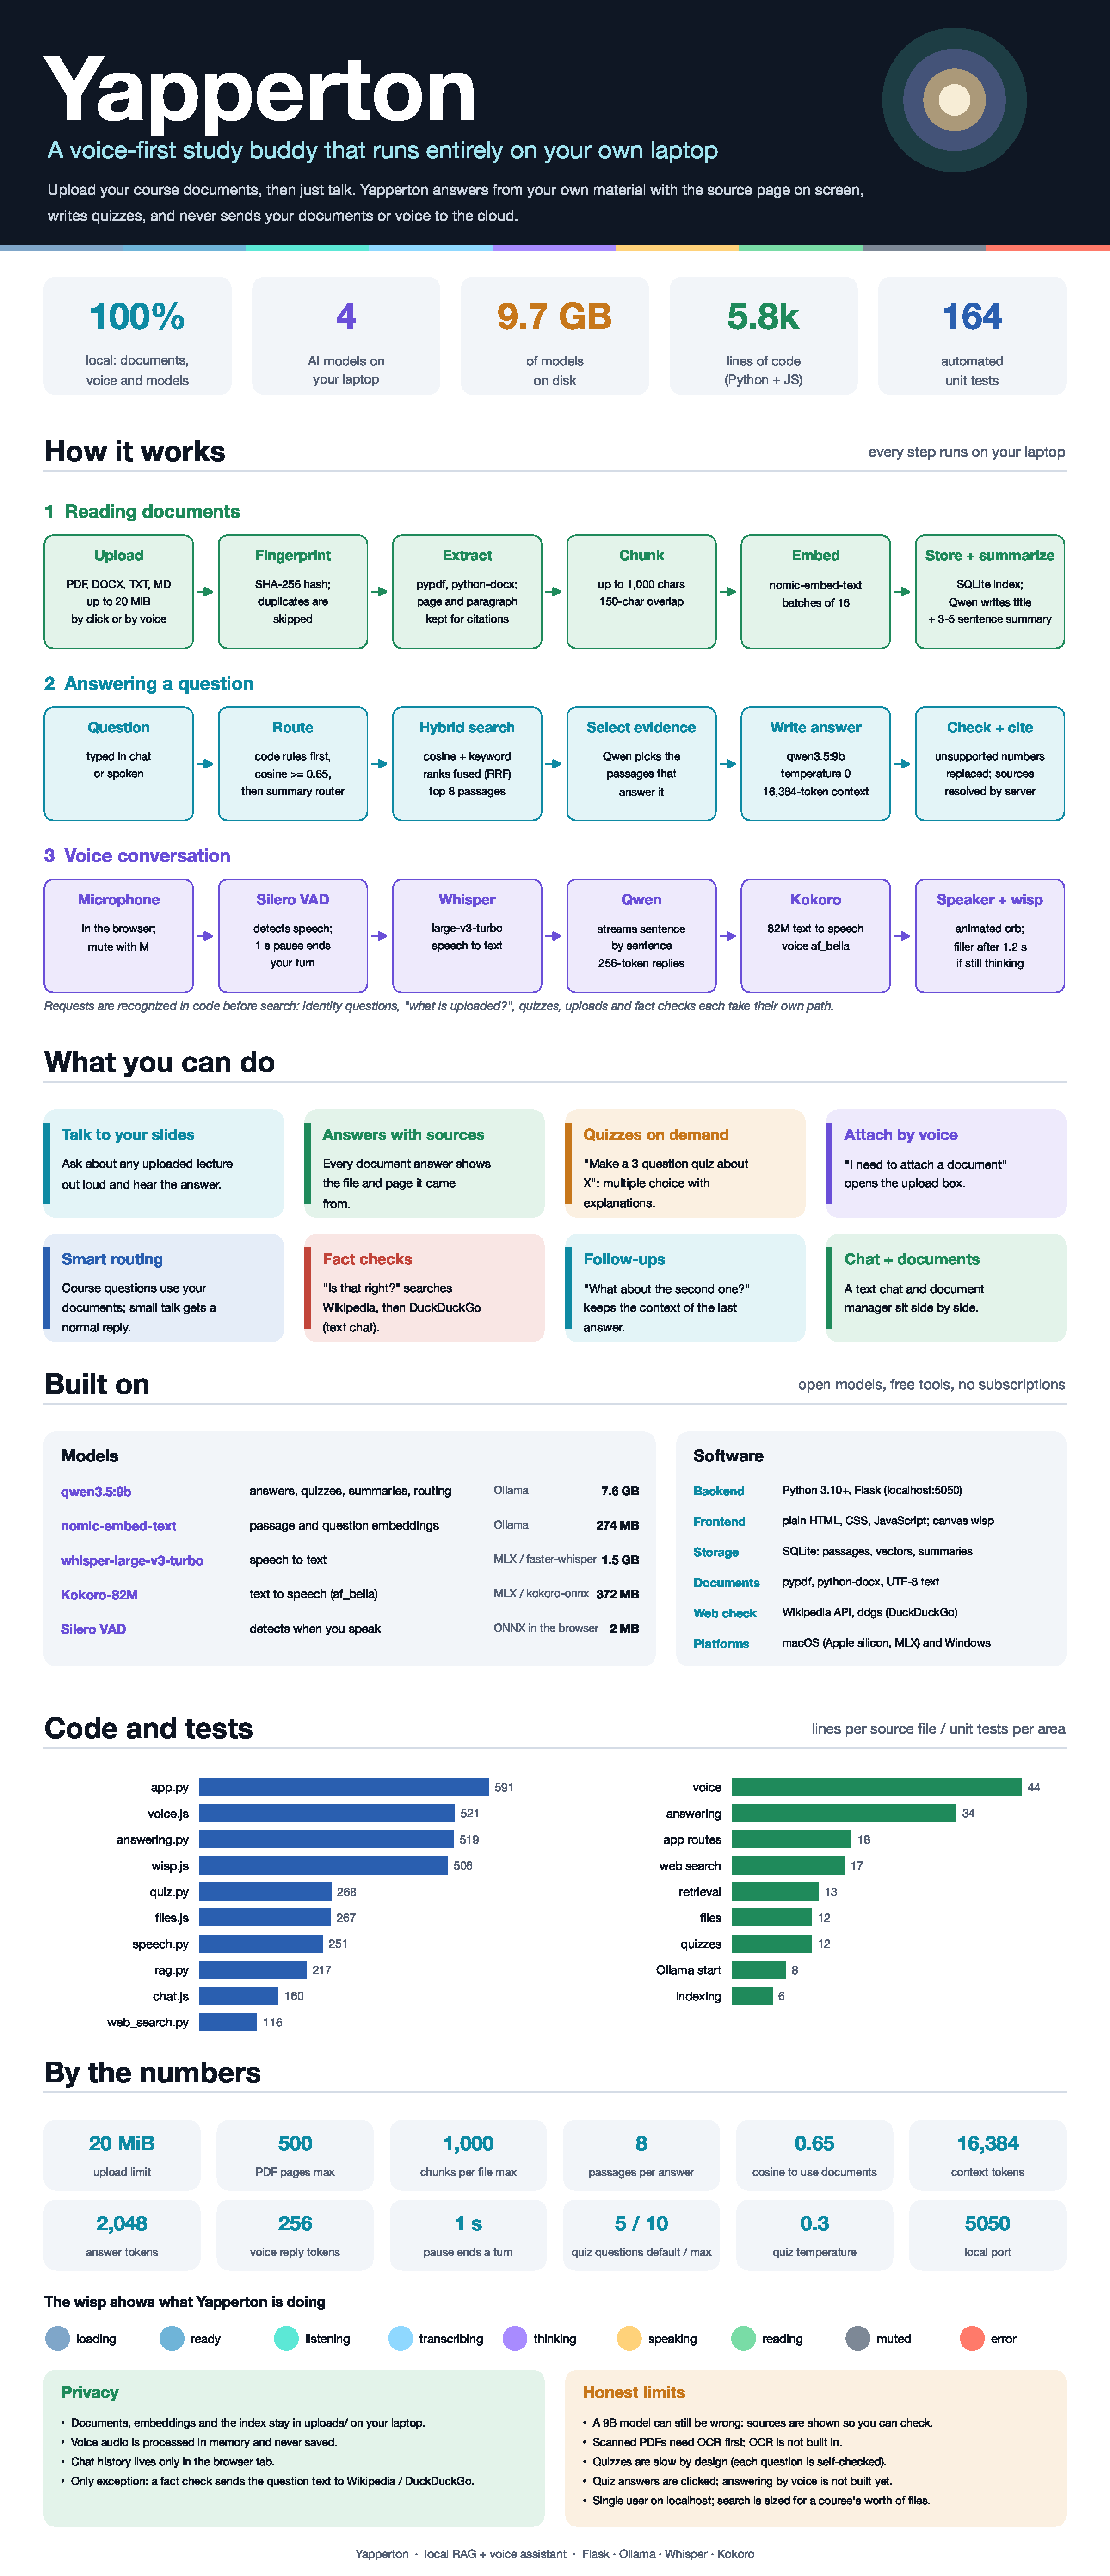
\includegraphics[height=0.92\textheight]{../yapperton_infographic.pdf}
  \caption{Yapperton infographic: pipelines, features, models, numbers and
           limits. A full-resolution PNG is in the repository
           (\texttt{report/yapperton\_infographic.png}).}
  \label{fig:infographic}
\end{figure}

\end{document}
